\documentclass{article}
\usepackage{amsmath}
\usepackage[letterpaper,showframe=false]{geometry} %"showframe=false" es necesario
\usepackage{tikz,tkz-tab} % Paquete para tablas de signos


\begin{document}


\begin{center}
\tikzset{t style/.style={style=thick}}    %Estilo l�nea continua
\tikzset{z style/.style={thick}}          %Estilo l�nea continua

                %Inicio de la figura
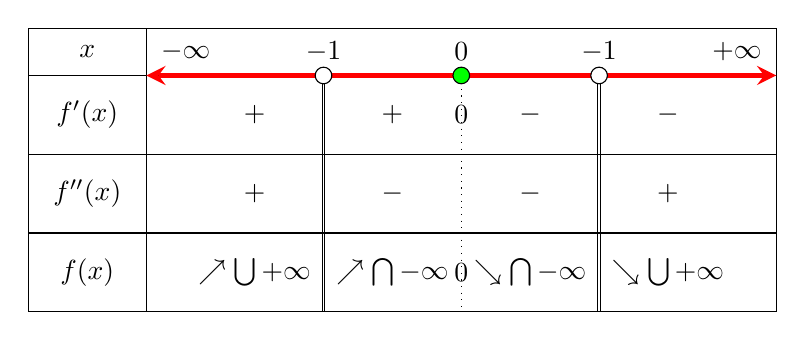
\begin{tikzpicture}[>=stealth]   % Estilo de flechas
                % "ldt" = ancho de 1ra columna, 1.5 = 1.5cm
                % "esplc"= espacio entre columnas
\tkzTabInit[lgt=1.5,espcl=1.75]  
                %1ra columna. El /0.6 es altura de 1ra fila = 0.6cm
                % Fila 0, n�meros en eje X.
{$x$ /0.6, $f'(x)$/1, $f''(x)$/1, $f(x)$/1} 
{$-\infty$,$-1$,$0$,$-1$,$+\infty$} 
                % Las otras filas de la tabla.
                %Inicia en Columna 2 y NO requiere $ $
                % Fila 1, "d" =  doble l�nea vertical, 
                %         "z" = l�nea vertical con "cero"
\tkzTabLine{ , + ,d, + ,z, - ,d, - } 
                % Fila 2
\tkzTabLine{ , + ,d, - ,t, - ,d, + } 
               % Fila 3
\tkzTabLine{ ,\nearrow \bigcup +\infty
           ,d, \nearrow \bigcap -\infty 
           ,z, \searrow \bigcap -\infty 
           ,d, \searrow \bigcup +\infty}

%Eje X : Desde nodo  T11 hasta nodo = T21 (Tji con j=col, i= fila).
\draw[line width=2pt,red,<->] (T11) to (T21); 
              % Punto blanco simula ser abierto; en nodo N21 (Nji)
\draw[fill=white](N21) circle(3pt); 
\draw[fill=green](N31) circle(3pt);
               % Punto blanco simula ser abierto; en nodo N41
\draw[fill=white](N41) circle(3pt); 
\end{tikzpicture}
\end{center}

\bigskip

Otro ejemplo\\

\bigskip
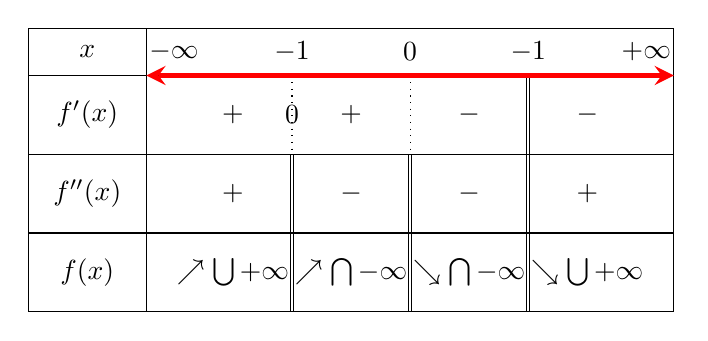
\begin{tikzpicture}[>=stealth] %Estilo de flechas
\tkzTabInit[lgt=1.5,espcl=1.5,deltacl=0.35] % "deltacl" = espacio adicional en columna 2 y la final
{ $x$ /0.6, $f'(x)$/1, $f''(x)$/1, $f(x)$/1} %1ra columna
{$-\infty$,$-1$,$0$,$-1$,$+\infty$} %fila 0
\tkzTabLine{ , + ,z, + ,t, - ,d, - } %1ra fila, "z" = l�nea vertical con '0'
\tkzTabLine{ , + ,d, - ,d, - ,d, + } %2da fila
\tkzTabLine{ ,\nearrow \bigcup +\infty
,d, \nearrow \bigcap -\infty 
,d, \searrow \bigcap -\infty 
,d, \searrow \bigcup +\infty}%3da fila
\draw[line width=2pt,red,<->] (T11) to (T21); %Col1Fil1 to Col2Fil1
\end{tikzpicture}

\bigskip
Otros ejemplos peque�os\\

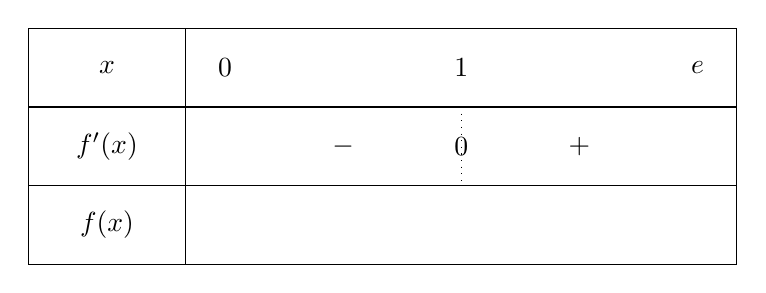
\begin{tikzpicture}
\tkzTabInit{$x$/1,$f'(x)$/1,$f(x)$/1}{$0$,$1$,$e$}
\tkzTabLine{,-,z,+}
\end{tikzpicture}

\bigskip
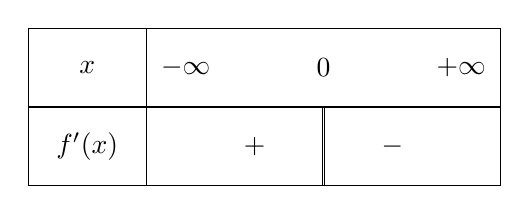
\begin{tikzpicture}
\tkzTabInit[lgt=1.5,espcl=1.75]%
{$x$ / 1,$f'(x)$ / 1}%
{$-\infty$,$0$,$+\infty$}%
\tkzTabLine{,+,d,-,}
\end{tikzpicture}

\end{document}